% Portrait version of architecture.tex (same content and colours) for a tall poster column.
% Natural size about 10.3 cm by 16.6 cm; smallest text 7 pt. Build: bash docs/assets/build.sh
\documentclass[11pt,border=4pt]{standalone}
\usepackage{times}
\usepackage[T1]{fontenc}
\usepackage[utf8]{inputenc}
\usepackage{xcolor}
\usepackage{tikz}
\usetikzlibrary{positioning,fit,backgrounds,arrows.meta,calc}
\definecolor{acc}{HTML}{1F3A5F}
\definecolor{locF}{HTML}{E3F1E0}\definecolor{locD}{HTML}{4E7D46}
\definecolor{modF}{HTML}{DDEAF6}\definecolor{modD}{HTML}{2F5D8A}
\definecolor{gtF}{HTML}{FCEBD0}\definecolor{gtD}{HTML}{A8690B}
\definecolor{psF}{HTML}{F7DADA}\definecolor{psD}{HTML}{A23B3B}
\definecolor{stF}{HTML}{ECE6F5}\definecolor{stD}{HTML}{6A5293}
\definecolor{lgF}{HTML}{EFEFEF}
\newcommand{\sm}[1]{{\fontsize{7}{8}\selectfont #1}}
\begin{document}
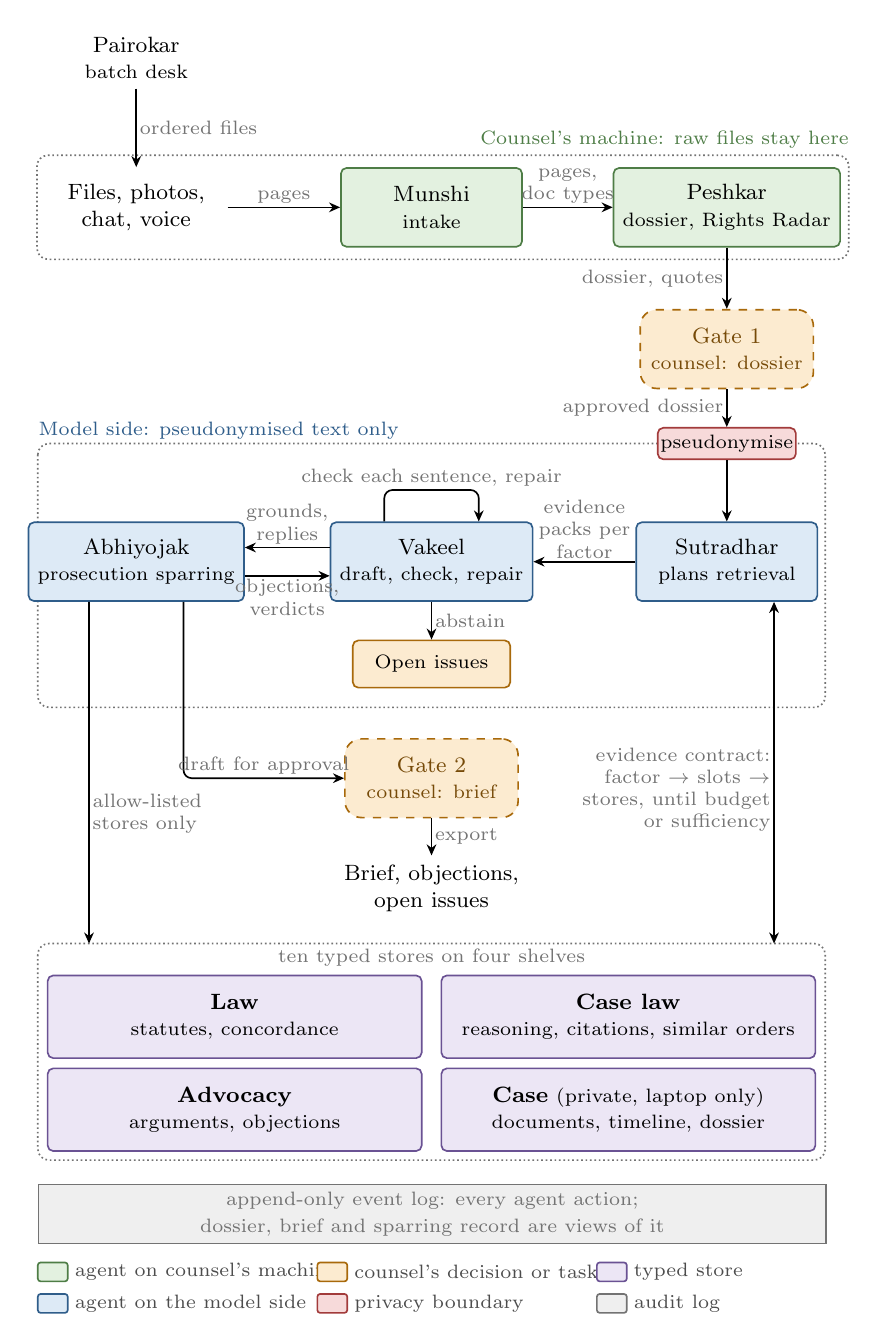
\begin{tikzpicture}[
  font=\fontsize{8}{9.5}\selectfont, >={Stealth[length=4pt,width=3.5pt]}, line width=0.6pt,
  loc/.style={ag, draw=locD, fill=locF},
  ag/.style={draw=modD, fill=modF, rounded corners=2pt, align=center, minimum width=2.3cm, minimum height=1.0cm},
  gt/.style={draw=gtD, fill=gtF, text=gtD!70!black, dashed, rounded corners=6pt, align=center, minimum width=2.2cm, minimum height=1.0cm},
  io/.style={align=center, minimum width=2.3cm, minimum height=1.0cm},
  sh/.style={draw=stD, fill=stF, rounded corners=2pt, align=center, minimum width=4.75cm, minimum height=1.05cm},
  lb/.style={font=\fontsize{7}{8}\selectfont, text=black!55, align=center, inner sep=1pt},
  fr/.style={draw=black!55, densely dotted, rounded corners=4pt}]
\def\ca{1.25}\def\cb{5.0}\def\cc{8.75}
% input
\node[io, minimum height=0.6cm] (pa) at (\ca,0.3) {Pairokar\\\sm{batch desk}};
% counsel's machine
\node[io] (in) at (\ca,-1.6) {Files, photos,\\chat, voice};
\node[loc] (mu) at (\cb,-1.6) {Munshi\\\sm{intake}};
\node[loc] (pe) at (\cc,-1.6) {Peshkar\\\sm{dossier, Rights Radar}};
\node[fr, fit=(in)(mu)(pe), inner ysep=0.15cm, inner xsep=0.1cm] (lap) {};
\node[lb, anchor=south east, text=locD, inner sep=0pt] at ([yshift=2pt]lap.north east) {Counsel's machine: raw files stay here};
\node[gt] (g1) at (\cc,-3.4) {Gate 1\\\sm{counsel: dossier}};
% model side
\draw[fr] (0,-4.6) rectangle (10.0,-7.95);
\node[lb, anchor=south west, text=modD, inner sep=0pt] at (0,-4.55) {Model side: pseudonymised text only};
\node[draw=psD, fill=psF, rounded corners=2pt, minimum width=1.75cm, minimum height=0.4cm, inner sep=1pt] (ps) at (\cc,-4.6) {\sm{pseudonymise}};
\node[ag] (su) at (\cc,-6.1) {Sutradhar\\\sm{plans retrieval}};
\node[ag] (va) at (\cb,-6.1) {Vakeel\\\sm{draft, check, repair}};
\node[ag] (ab) at (\ca,-6.1) {Abhiyojak\\\sm{prosecution sparring}};
\node[ag, draw=gtD, fill=gtF, minimum width=2.0cm, minimum height=0.6cm] (oi) at (\cb,-7.4) {\sm{Open issues}};
% approval and output
\node[gt] (g2) at (\cb,-8.85) {Gate 2\\\sm{counsel: brief}};
\node[io, minimum height=0.75cm] (out) at (\cb,-10.25) {Brief, objections,\\open issues};
% stores
\draw[fr] (0,-10.95) rectangle (10.0,-13.7);
\node[lb, anchor=north] at (5.0,-10.97) {ten typed stores on four shelves};
\node[sh] (s1) at (2.5,-11.88) {\textbf{Law}\\\sm{statutes, concordance}};
\node[sh] (s2) at (7.5,-11.88) {\textbf{Case law}\\\sm{reasoning, citations, similar orders}};
\node[sh] (s3) at (2.5,-13.06) {\textbf{Advocacy}\\\sm{arguments, objections}};
\node[sh] (s4) at (7.5,-13.06) {\textbf{Case} \sm{(private, laptop only)}\\\sm{documents, timeline, dossier}};
\node[draw=black!55, fill=lgF, minimum width=10cm, minimum height=0.75cm, anchor=north west, inner sep=0pt, align=center, text=black!55] (lg) at (0,-14.0) {\sm{append-only event log: every agent action;}\\\sm{dossier, brief and sparring record are views of it}};
% flow arrows
\draw[->] (pa) -- node[lb, right] {ordered files} (in);
\draw[->] (in) -- node[lb, above] {pages} (mu);
\draw[->] (mu) -- node[lb, above] {pages,\\doc types} (pe);
\draw[->] (pe) -- node[lb, left] {dossier, quotes} (g1);
\draw[->] (g1) -- node[lb, left] {approved dossier} (ps);
\draw[->] (ps) -- (su);
\draw[->] (su) -- node[lb, above] {evidence\\packs per\\factor} (va);
\draw[->] ($(va.west)+(0,0.18)$) -- node[lb, above] {grounds,\\replies} ($(ab.east)+(0,0.18)$);
\draw[->] ($(ab.east)+(0,-0.18)$) -- node[lb, below] {objections,\\verdicts} ($(va.west)+(0,-0.18)$);
\draw[->, rounded corners=3pt] ($(ab.south)+(0.6,0)$) |- node[lb, above, pos=0.75] {draft for approval} (g2.west);
\draw[->] (g2) -- node[lb, right] {export} (out);
% Vakeel check-and-repair loop and abstention exit
\draw[->, rounded corners=3pt] ($(va.north)+(-0.6,0)$) -- ++(0,0.4) -- ++(1.2,0) -- ($(va.north)+(0.6,0)$);
\node[lb, above] at ($(va.north)+(0,0.4)$) {check each sentence, repair};
\draw[->] (va) -- node[lb, right] {abstain} (oi);
% stores
\draw[<->] ($(su.south)+(0.6,0)$) -- node[lb, left, align=right, pos=0.55] {evidence contract:\\factor $\to$ slots $\to$\\stores, until budget\\or sufficiency} (\cc+0.6,-10.95);
\draw[->] ($(ab.south)+(-0.6,0)$) -- node[lb, right, align=left, pos=0.62] {allow-listed\\stores only} (\ca-0.6,-10.95);
% legend
\begin{scope}[shift={(0,-15.12)}]
\foreach \i/\f/\d/\t/\x/\y in {0/locF/locD/agent on counsel's machine/0/0, 1/modF/modD/agent on the model side/0/-0.4, 2/gtF/gtD/counsel's decision or task/3.55/0, 3/psF/psD/privacy boundary/3.55/-0.4, 4/stF/stD/typed store/7.1/0, 5/lgF/black!55/audit log/7.1/-0.4}
  {\node[draw=\d, fill=\f, rounded corners=1pt, minimum width=0.38cm, minimum height=0.24cm, inner sep=0pt] (k\i) at (\x+0.19,\y) {};
   \node[lb, anchor=west, text=black!70] at ([xshift=1pt]k\i.east) {\t};}
\end{scope}
\end{tikzpicture}
\end{document}
